\documentclass[twocolumn,14pt]{extarticle}
\usepackage{hyperref}
\usepackage{listings}
\usepackage{graphicx}
\usepackage{lscape}
\usepackage{dirtytalk}
\usepackage{color}

\definecolor{lightgray}{rgb}{.9,.9,.9}
\definecolor{darkgray}{rgb}{.4,.4,.4}
\definecolor{purple}{rgb}{0.65, 0.12, 0.82}

\lstdefinelanguage{JavaScript}{
  keywords={typeof, new, true, false, catch, function, return, null, catch, switch, var, let, const, if, in, while, do, else, case, break},
  keywordstyle=\color{blue}\bfseries,
  ndkeywords={class, await, export, boolean, throw, implements, import, this},
  ndkeywordstyle=\color{darkgray}\bfseries,
  identifierstyle=\color{black},
  sensitive=false,
  comment=[l]{//},
  morecomment=[s]{/*}{*/},
  commentstyle=\color{purple}\ttfamily,
  stringstyle=\color{red}\ttfamily,
  morestring=[b]',
  morestring=[b]"
}

\lstset{
   language=JavaScript,
   backgroundcolor=\color{lightgray},
   extendedchars=true,
   basicstyle=\footnotesize\ttfamily,
   showstringspaces=false,
   showspaces=false,
   numbers=left,
   numberstyle=\footnotesize,
   numbersep=9pt,
   tabsize=2,
   breaklines=true,
   showtabs=false,
   captionpos=b
}

%AudioToken: a sound based authenticator
\title{CO880 - Project dissertation}
\author{Arthur Knoepflin\\\href{mailto:adbk2@kent.ac.uk}{adbk2@kent.ac.uk}}

\begin{document}
\onecolumn
\maketitle
\clearpage
\tableofcontents
\clearpage
\listoffigures
\twocolumn

\section{Introduction}
In our today's world, computer security become more and more important. This is due to the fact that we are continually computerizing tasks, activities or administration. In order to keep a good security, numerous web platforms have implemented a second authentication system, also called multi-factor authentication. This mechanism does make the connection of the user possible only after validating two different authentication systems (for example password + code received by SMS). Paradoxically, a vast majority of users are not using these new authentication schemes. According to Sanchari Das et al., this lack of general public acceptation is due to the boring aspect of MFA \cite{das2019mfa}, their paper explains that, from a user perspective, the effort it takes to setup and use a second authentication factor is not worth the amount of security it brings. Their recommendation is to provide a more elegant and effort-less MFA technology that do not depends on the device used (laptop, smartphones, ...). So, in this paper we will propose a new easy and pleasant second authentication mechanism.

This new authentication mechanism must be simple to understand, must work anytime in any situation, must be transparent to use for the users and must work on hardware that the users already have. Statistics show us that 71 millions peoples are using a cellular phone in United Kingdom, which represents 107\% of the population. Also, 77\% of the cellphones are smartphones \cite{comarketing_2019}. Therefore, our new authentication mechanism will use a smartphone to work because we will be able to cover more than 80\% of the population.

The second challenge is to find a mechanism that can authenticate a user and that is transparent for the user. This mechanism must work with the capabilities offered by smartphones. Most recent smartphones are equipped with a lot of sensors and security device like fingerprint reader, but using these will reduce the compatibility of our authentication system. Also we cannot use any of the internet features offered by smartphones as they will reduce the usabilty, indeed it may happen that the user does not have access to the internet. For our new authentication mechanism we will use the microphone and the speaker of the smartphone as they are necessarly implemented in every smartphones and in a majority of computers. The goal of this authenticator will be to exchange data between the computer where the user wants to authenticate itself and a smartphone where the user have the authenticator application installed. The data will be exchange through audio, using the speakers as emitter and the microphones as receiver. This new authentication mechanism is named AudioToken.

In the \hyperref[sec:passinfinity]{first section} of this dissertation I will briefly explain what is PassInfinity and how it works, in the \hyperref[sec:audiotoken]{second section} I will explain how the authenticator works. In the \hyperref[sec:implementation]{third section} I will describe how we can implement our own data transmission system. In the \hyperref[sec:limitationsfurtherwork]{next section} I will extend the subject of this dissertation to see what are the limitations and what could be done next. Finally, in the \hyperref[sec:conclusion]{last section}, I will conclude the dissertation.

\section{PassInfinity}
\label{sec:passinfinity}
This new authentication mechanism is part of a wider project named PassInfinity (\href{https://www.passinfinity.com/}{https://www.passinfinity.com/}). PassInfinity is an all-in-one authentication framework, it is universal, flexible, reconfigurable, scalable and user-centric authentication system. PassInfinity is held under the form of a password manager but instead of storing the users password in a database, like a standard password manager, it uses modules to compose user passwords. Each modules of the PassInfinity project must work like a pure function, which means that for the same input, the same output must be produced (See appendix \ref{appendix:sec:purefunction}). There are a multitude of modules available, the users can choose which modules they want to use. The final password is then a concatenation of the output of each module the user have chosen.

Each module is divided in different categories according to there authentication factor type. There are 4 authentication factor types different compatible with PassInfinity:
\begin{itemize}
\item Knowledge-based, what you know. For example: passwords.
\item Possession-based, what you have. For example: smart-cards, bank security token, etc.
\item Inherence-based, who you are. For example: fingerprint reader, iris scanner, etc.
\item Context-based, where you are. For example: ip location, gps location, etc.
\end{itemize}
The users are encourage to use multiple modules as it will strengthened their password security. 

In order to enforce a minimum security policy, websites that implement PassInfinity can decide an authentication policy. This policy constrains the number of modules used for each authentication factor type. A policy can, for example, force a user to use at least one knowledge-based module and two possession-based modules.

\subsection{Functional use}
From a user point of view, PassInfinity is really easy to use. When a user want to signup on a website, he will need to acces to register page as usual. The usual password input would be replaced by the PassInfinity input. In this input the user would be given the choice of which modules he want to use. The user will then have to remember the modules he used and the order. Obviously, he will also have to remember the inputs of the knowledge-based modules. The password transmitted to the server for the registration process is the concatenation of the outputs of all the modules he has used. Further treatment can also be added at the time of the concatenation, like a hash-and-salt algorithm.

Once the user registered, he can also login itself easily. The process is the same as the registration, the user will need to go to the sign in page. The usual password input would be replaced by the PassInfinity input. Exactly like the registration process, the user would be given the choice of modules. So that he can reconnect to the site, he must use the same modules in the same order. Once finished the output of the modules are concatenated, further treatment can also be added at this step, and then is sent to the server.

\subsection{Advantages}
PassInfinity solves multiple issues regarding MFA acceptability. Therefore it is a good solution to consider for improving the cyber security level of the general public.\linebreak
There are however few differences with classical MFA solutions.
\begin{itemize}
\item PassInfinity is way more flexible than classical 2FA as the user can freely choose which authenticator he wants to use and in which order.
\item PassInfinity may leave the possibility to the user to only one authentication factor. Therefore it can be implemented on a website without interfering with the current authentication flow of the users.
\item PassInfinity can cover all authentication factor type (knowledge-based, possession-based, ...) in one implementation.
\item PassInfinity is a one step authentication process, which means that even if there are multiple authentication factor, they can work altogether. For example an authentication factor can use the result of another one.
\item PassInfinity is highly reconfigurable and scalable, new modules can be easily added without modifying the back-end architecture and without modifying the user experience.
\item PassInfinity is fully backward compatible, the concatenation of the ouput of the modules still produces a text that can be used as password. Therefore it does not need to change the database system that hold passwords.
\end{itemize}

\subsection{Technical functionning}

Figure \ref{appendix:fig:passarchitecture} shows the architecture of PassInfinity. The base components are represented in the green area and the module components are represented in the beige area. This figure shows how much the base components are independant from the modules, indeed there are no direction connection, which means that the PassInfinity modules can work indepently of the base components implementation. Even if the current most use base component implementation is the textual password (save a small text fragment inside a database), PassInfinity could work with any other system. The base components are separated from the modules for keeping the base implementation changeable without having to change the modules.

Each component are further divided in two parts, the front-end, on the left of the figure, and the back-end, on the right of the figure. The front-end components represent all the parts the user can see and interract with, this is generally considered as the graphical user interface. The back-end components represent all the parts that the user cannot see, this is generally the parts that run on a server. Each parts can communicate with each other using Internet.

The architecture of PassInfinity has been designed so it can be implemented in several ways. For example, it can be implemented as a \textit{fat client}, like a password manager for Windows or Android. Or else, the system could be developed so that it can run in a browser, like a \textit{thin client}.

\subsubsection{Base components}

There are three components in the baseline components, the \textit{baseline editor}, the \textit{baseline module} and the \textit{baseline data}. The baseline editor is the only component in the front-end part, the component handle the base user interface of the PassInfinity input. It allows the modules to be displayed to the users. The baseline module is the back-end component that receives all the output of the modules and then compose a final password. This is also this module that check if a given password is the correct password for a given user. The baseline data is a storage systems (usually a database) that will store the hash version of the user's password and some other settings. The implementation of the base components depends of the system on which it is launched.

\subsubsection{Modular components}

There are also three components in the modular components, the \textit{PassInfinity modules}, the \textit{password policy controller} and the \textit{module data} (named \textit{New Data} on the figure). The PassInfinity modules are often only on the front-end side, but can contain sometimes a backend part, usually for handling the database communication. The modules are responsible of the creation of a part of the final password, they take zero, one or multiple input(s), and produce one output. The module data is a storage system (usually a database) that can hold information for the PassInfinity modules. This storage system must not store any passwords of any kind but only store necessary information for the modules to work. The modules must be platform free, which means that they must work on any implementation and that is up to the base components to make them compatible with the system.

\subsubsection{Password policy controller}

Password policy controller is a special component of the modular components. It allows website owners to control the minimum security they want on their platform. This module register which modules and which authentication factor type the user is using. According to a policy, given and set in the back-end part, the password policy controller can refuse a password that do not match the minimal requirement. This component help define how secure the generated passwords are. 
\\
\\
\\
Now that the working principle of PassInfinity has been presented, we will see how we can create and implement a module that use audio to authenticate users.

\section{Audio token}
\label{sec:audiotoken}
As introduced in the first section, the goal is to create an authenticator that use the microphone and the speaker of either a phone or a computer. The difficulty here is to keep this authenticator functional in any circumstances, even when there is no network available.

After some research it appears that there are already some authenticators that use audio. One of them is named \textit{Sound-Proof} \cite{sound_proof}. In their solution, Nikolaos Karapanos et al. use the microphone of both the computer and the smartphone to record a short audio sample. These two audio samples are then compared to each other, and if the recordings match, the access is granted. The idea behind this authenticator is that the computer and the smartphone of the user must be nearby so that they can record the same audio sample. If this systems seems a great idea it has two major drawbacks, firstly it requires Internet to work. Indeed it uses an internet connection to exchange the audio sample between the smartphone and the computer, and it also uses internet to synchronise the start of the recording. The second drawbacks is that this system only works well in an noisy environment. Because of the operating principle, if the user is located in a quiet room there are no specific markers in the audio recording to match, whereas if the user located close to people talking, the conversation will bring specific markers to match.

\subsection{Working principle}
\label{sec:audiotoken:workingprinciple}
Even if the \textit{Sound-Proof} paper brings many good elements, the final solution is not satisfying. After few more searches I've come to another solution: Audio Token. The idea of Audio Token is to transmit data from the computer to the smartphone or vice versa using the speaker and the microphone of the devices. The speaker will be the transmitter medium and the microphone will be the receiver medium. The working principle of this authenticator is very simple, the device that want to authenticate itself will emit a challenge and the device that must verify the identity of the owner will catch this challenge, will compute a response and then will send it back.

There are many advantages to this authenticator, firstly the workflow is highly transparent for the user as the only step he will have to do is to make the validator device listening. Secondly this authenticator can work in almost any conditions, with or without Internet and in a noisy or a quiet environment. Thirdly, this mechanism only use very common peripherals on smartphones and computers, consequently this authenticator will be able to function on many devices. It will also be able to operate seamlessly whatever the brand of equipement, the operating system or the platform used. And lastly, one of the main advantage it brings is the security, as the audio crosses wall very poorly, the validator device will need to be physically near the computer.

\subsection{Architecture}
As seen on the figure \ref{appendix:fig:audioarchitecture}, there are three main steps in this authenticator.

The first step is the initial broadcast of the challenge. This step involves both the computer and the validator device (smartphone on the figure). The choice of the challenge is left to the computer. The challenge is composed of a short text but for the sake of consistency, it's preferable to keep the same length for the challenge. With a challenge of different size, the encoded audio would be longer. Therefore the challenge will be hashed before being encoded. The choice of the hash algorithm is non important but it must be the same everywhere once chosen. In our implementation we will SHA-256, a strong cryptographic hash function developped by the NSA \cite{wiki:SHA-2}. This hash function produces a 256 bits stream, that is to say 32 bytes. Once the challenge chosen and hashed, it is encoded and sent to the smartphone (validator device) using audio.

The second step is the compute stage, in this step the goal is to calculate a new challenge (the response) from the intial challenge. This step only involves the validator device (smartphone). This calculation must have the same properties as a pure function (for example see section \ref{appendix:sec:purefunction}), it must have the same output for the same input. However, the output must be unique per devices in order to authenticate the user. Therefore we need a function that consumes an input and a key and produces an output, for the same input and key we must obtain the same output. In our implementation we will use a HMAC function and more specifically a HMAC-SHA256 \cite{wiki:HMAC}. This HMAC function also produces a 256 bits stream, that is to say 32 bytes. The input provided to the HMAC function will obviously be the challenge received in the first step. The key supplied to the HMAC function will be a random string generated when the PassInfinity application is installed, the key must always be the same otherwise it will not be possible to verify the identity of the user.

The third and last step is the broadcast of the response. Again, this step involves both the computer and the validator device. Once the response has been computed in the second step, it is send back to the computer using audio. That means that the computer and the smartphone are alternatively receiver and emitter. Once the computer has received the data, the response is the ouput of the module, therefore it will then be used by PassInfinity to compose the final password of the user.

As explained in this section, the choice of the initial challenge is crucial as it will determine the result of the whole process. Due to the current architecture of PassInfinity, so that the user can log in again, the challenge must be the same for the same website, therefore I use in my implementation the hostname of the website. 
\\
\\
\\
The whole technical process of Audio Token is now explained, however there is still a grey area, how can we exchange 256 bits between a computer and a smartphone using only audio. In the following section we will see the state of the current technologies and methods.

\section{Literature review}
In the previous section we have seen that the real challenge in this new authenticator will be to carry data through audio. Therefore, before trying multiple implementation, we will search who and what is using audio to transmit data.

\subsection{Data transmission techniques}
In their article, Anil Madhavapeddy et al refer to audio as the \say{the forgotten wireless technology} \cite{1495392}. They propose multiple usage of audio to transmit data, for example exchange a pin code required to initiate a bluetooth connection, exchange small data while having a conversation on a phone, or else, exchanging Internet rendezvous information for transferring complexe data. The most interseting part of this article is the explanation of the mechanism they use to exchange such data through audio. They propose four different methods:
\begin{itemize}
\item dual-tone multifrequency (DTMF)
\item on-off keying (OOK)
\item inaudible data transmission
\item melodic data transmission
\end{itemize}

Firstly, dual-tone multifrequency, or DTMF, is the system used in the conventional telephony to compose the numbers when dialing someone. This system is based on a combination of two frequencies, there are two times 4 frequencies, therefore we can send up to 16 different values (4 * 4). This system has been developped for sending the 10 numbers, the "*", the "\#" and four buttons "A" "B" "C" and "D" (See figure \ref{appendix:fig:dtmfkeypad}). Using DTMF encoding, they claimed to achieve a bitrate of 20 bits per second.

Secondly, on-off keying, is a system that represents digital data as the presence or the absence of a carrier wave. The carrier wave is a high frequency wave decided between the emitter and the receiver, we use a hight frequency instead of the original signal because it allows us to send the data with a much higher range. When we want to send a binary one, we emit the high frequency, when we want to send a binary zero, we stop the broadcast of the carrier wave. Using on-off keying they obtained a data rate of 251 bits per second.

Thirdly, inaudible data transmission, is a variant of the on-off keying but using an ultra-sound (between 16 kHz and 100 kHz) for the carrier wave. The advantages of using such frequency for the carrier wave is that they are inaudible for humans. In theory, a human car hear sound between 20 Hz and 20 kHz, but these values are different for each person depending on the age and lifestyle. In the arcticle, they choose a frequency for the carrier wave of 21.2 kHz. Using this technique they achieved a bitrate of 8 bits per second.

And finally, melodic data transmission, is another variant of on-off keying that use 4 different carrier frequencies. The 4 frequencies are defined from a music mode, they are used according to a pattern called a theme. This pattern has been specifically generated so that it is pleasant to hear. Each use of a frequency represents 2 bits. Using melodic data transmission they claimed to obtain a maximum data rate of 83 bits per second. Unfortunately, at this bitrate the melody is played to quickly and become unpleasant to hear, therefore the authors recommand not to exceed 14 bits per second.

At first glance, the on-off keying seems to be the most interesting encoding method. It can provide us with a "high" bitrate, 251 bits per second is almost sufficent to send an entire SHA256 in one second. The DTMF method also looks promising, even if the bitrate is not as good as the on-off keying method. The inaudible data transmission is unfortunately unsufficent for us, with 8 bit per second it would take 32 seconds to send one SHA256. Similarly, the melodic data transmission will not be considered furthermore, even if the bitrate is okay, this method would require music knowledge that I unfortunately don't have.

\subsection{Passband modulation}
As the on-off keying method seems to be the most interesting method, we will firstly explore this method. This method is part of passband modulation, it is the process of varying one or multiple properties of a periodic waveform, named carrier wave, according to a signal that must be send. Passband modulations are designed to be used with radio-frequency, however, audio is in many way similar to radio-frequency. Both use frequency to transmit information, one is with the oscilation of an electric charge and the other is with the movement of the air. Therefore some passband modulation can be applied with audio. There are two major types of passband modulation, analog modulation where the data to send are analog and the digital modulation where the data to send are binary. Analog modulation is mostly famous for there radio usage, like the FM (Frequency modulation), a passband modulation where the frequency of the carrier wave is changed according to the signal to be sent, and AM (Amplitude modulation), another passband modulation where the amplitude of the carrier wave is changed according to the signal to be sent. In our case analog modulation is not a good solution as the data we need to send (SHA-256) are represented under a binary form, therefore we will use digital modulation. 

There are numerous digital modulation but in this paper we will only look at the four most famous: Amplitude shift keying (ASK), Phase shift keying (PSK), Frequency shift keying (FSK), On-off keying (OOK).
\begin{itemize}
\item ASK is a passband modulation where the amplitude of the carrier wave varies according to the signal to sent (see figure \ref{appendix:fig:ask}). If we want to send a binary 0, we will reduce the amplitude, on the contrary, we will increase the amplitude if we need to send a binary 1. This modulation works well for a radio signal but would be very hard to implement using audio. In audio, the modification of the amplitude result in a modification of the volume, increasing the amplitude increase the volume. Data transmission is highly sensible to volume changes, if the user change the volume of the emitter or moves his smartphone or his computer during the transmission, that will produce volume changes. Therefore we cannot rely on ASK to transmit our signal.
\item PSK is another passband modulation where the phase of the carrier wave changes in function of the signal to be sent (see figure \ref{appendix:fig:psk}). When we want to send a binary 1 we emit our carrier wave in the positive sense (trigonometric direction), and for a binary 0, we emit our carrier wave clock-wise. Unfortunately for us, PSK requires a very high level access on the microphone and the speakers, as we will have to implement our data transmission mechanism inside a browser, it is very unlikely that we achieve to get such a high level access on the hardware of the computer or the smartphone. Moreover this modulation mechanism is very complex to implement. That is why we are not going to use this modulation technique.
\item FSK is a digital modulation where the frequency of the carrier wave is changed according to the signal to be sent (see figure \ref{appendix:fig:fsk}). For sending a binary 0, we set the carrier wave to a specific frequency, and for sending a binary 1, we set the carrier wave to another frequency. This modulation techniques works very well for radio communication but also with audio. In audio, a change of the carrier wave frequency will result in an change of pitch of the audio signal, this change of pitch can be easily detected using a simple microphone. Also, the frequency of a sound is not affected by any movement of any kind, it is therefore one of the most promising passband modulation.
\item As explained in the review of the article, OOK is another digital modulation, similar to FSK, where we emit or not the carrier wave according to the signal we want to send (see figure \ref{appendix:fig:ook}). If we send a binary 1, we emit the frequency on the carrier wave, and if we want to send a binary 0 we stop the emission of the frequency on the carrier wave. This solution is very similar to FSK as in both of these modulation, we change the frequency of the carrier wave, therefore OOK enjoys the same advantages as FSK. However, as OOK only use one frequency it is slithgly easier to implement, this is why we are going to continue the research with OOK.
\end{itemize}

Now that we know that FSK or OOK could be an intresting method to exchange data through audio, we need a paper that can prove the theory. In 2018, Francis Iannacci and Yanping Huang write a paper about a system of their invention, ChirpCast \cite{ChirpCast}. ChirpCast is a system that can broadcast network access key through audio, the goal is to provide an easy system for smartphone and laptop to connect to public Wi-Fi, like in restaurant, library or in other public places. The advantages of their system is that the audio cross very poorly the walls, therefore the network access key can only be "heard" inside the room we want to give access to the Wi-Fi. In their paper they claimed to achieve a bitrate of 200 bit/s using some passband modulation techniques. Their final solution for the data transmission is a variation of phase shift keying (PSK) nammed differential phase shift keying (DPSK). The operating principle is very similar, it is however a bit more easier to implement. The major difference come with the change of phase, instead of changing the phase of the carrier wave for indicating a binary 1 or 0, we simply add $\pi$. For sending a binary 1, we add $\pi$ to the current phase, and for sending a binary 0 we add 0 to the current phase. Unfortunately for us, as explained previously it is not possible for our system to use PSK or even DPSK.

However, the ChirpCast paper is still intersting for our data transmission mechanism as in the section 3.1 they implement a frequency shift keying (FSK). For their FSK they have chosen 18 kHz to be the frequency for a binary 0 and 18.25 kHz for a binary 1. Both of these frequency are not ultra sound frequency (superior to 22 kHz) but they are most probably not audible for the majority of humans. In addition to their system, in order to synchronise the emiter and the receiver, they use another signal that works as a clock. At each time they send a bit, whether it is a logical 1 or 0, they alternatively emit two other frequencies, 18.5 kHz and 18.75 kHz. This mechanism allows the receiver to synchronise the reception to the emitter and to easily decode consecutive bit. They take advantage of the stereo, available in almost every laptops and speakers, to emit their two signals. On the left channel they send the FSK and on the right channel they send the clock. Even if it is a good idea to separate the audio channel for the signal and the clock, we will not be able to use this mechanism in our data transmision as it needs to work on smartphones and the majority of smartphone have only one speaker. Therefore, in our implementation, we will send the FSK and the clock on both channel.

\subsection{DTMF}
Another interesting mechanism for our data transmission is DTMF. DTMF stands for Dual-Tone MultiFrequency, as explained in a previous section it is the system used in the conventional telephony to compose the numbers when dialing someone. It is also used in automated vocal server where you have to press a number on your keypad to access a submenu. This mecanism allows to encode up to 16 values. The system is quite simple, it consists of a two-dimensional matrix of size 4 by 4 (See table \ref{appendix:table:dtmf}). For encoding a value, we have to get the "abscissa" and the "ordinate" of the value in the matrix. Let's assume we want to encode the value "6" from the keypad, the "ordinate" (the y) is 2, so the frequency that we read is 770 Hz and the "abscissa" (the x) is 3, so the frequency that we read is 1477 Hz. The two frequencies that we get for "6" are 770 Hz and 1477 Hz, for sending our value we just need to emit both frequency at the same time. For our purpose, we will remap the DTMF keypad for sending hexadecimal values between 0 and F (from 0 to 9 and A to F, 16 values). In some way we can see DTMF as a variant of FSK.

One of the advantage of this encoding mechanism is that we can send up to 4 bits at the same time ($\log_2 16 = 4$). For our data transmission system, the idea would be to split in half each byte we have send (32 for SHA-256), this would give our 4 bits, we will just have to encode them and to emit them. Therefore it will take us 2 tones to emit 1 byte. Splitting in half a byte is quite easy with most of programming language. The idea is to use a binary mask, \textit{0b1111} we can get the 4 last bits and with \textit{0b11110000} we can get the 4 first bits, we also have to bit shift 4 to the right to get a value between 0 and 15.

Once again we need a paper to prove our theory. In 2004, two peoples from the university of Washington, Tho Nguyen and Linda Bushnell, conducted a study on the fesability to use DTMF for communications between robots \cite{DTMFfeasibility}. This paper describes the design and implementation of several experimentation to answer the question. Their experimentations use two mobile robots equiped with 4 wheels, an Handy Board (electronic controller), a microphone and a speaker. They use DTMF to send simple commands like go forward, go backward, turn left, acknowledge, etc. In the first experimentation they set a robot to remain static, this robots is in charge to give order to the other robot. In the second experimentation, both robots are moving, the order are transmitted alternatively. The major issue they encountered into their experiments is the transmission distance, indeed, due to the movement of the robots and their relative orientation, the communication is quickly non-functional as the audio is not properly received. The conclusion of the paper is that DTMF is not suitable for robots communication.

This paper raise interesting question, notably on transmission distance. Indeed, the point that made the author of the paper say that DTMF is not suitable for the communication is the transmission distance. This limitation is mostly due to the fact that they use moving robots, we will not be concerned by this problem in our authentication process as the validator device (smartphone) must remain static while proceeding to the authentication. Moreover the short transmission distance is an advantage for our system because it will strengthen the security of our authenticator. Therefore we can still considered DTMF as a good solution for our data transmission mechanism.

\subsection{Conclusion}
In this section we have seen multiple methods to transmit data using audio, we have seen that radio-frequency and sound are very similar and that some modulation techniques can be used with the sound. Using an intresting article from the IEEE Pervasive Computing journal we have identified two different methods, one using passband modulation and another one with DTMF. This article also indicates that passband modulation seems to be the most promising techniques, with the highest bitrate. That's why we are going to use it firstly, if for any reason we are unable to proceed with this technique, we will fallback to the DTMF method.

In the next section we will see how to implement our data transmission method into a web browser.

\section{Implementation}
\label{sec:implementation}
As seen in the previous section we are firstly going to implement an On-Off keying. One difficulty is that it must mork inside a web browser, indeed, since PassInfinity is integrated inside a web pages through its input, every PassInfinity module must work in it. Therefore every code produced for the module must be in javascript and must use web browser APIs. 
This project is split in two part, the PassInfinity module (which runs on the computer) and the validator device (which most probably runs on the user smartphone), the code for the validator device does not need to be executed inside the web browser, it could be implemented using native language (Java for Android and Swift for iOS), but since we are going to code a version for web-browser, we will re-use the code for avoiding code duplication.

In this section we will firstly see how we can emit a sound and read the microphone inside a web browser. Secondly we will implement a On-Off keying and a DTMF data transmission mechanism. And thirdly we see how we can use a HMAC in a browser.

\subsection{Web Audio API}
So, since we need to implement our data transmission through audio inside a web browser, we are going to need an API to communicate with the speaker and the microphone of the computer. Indeed, for safety reason, a web browser is highly isolated from the hardware capabilities. However, nowadays the majority of web browser are providing high level API to communicate with the hardware, this is the case for the microphone and the speaker of a device. If we want to emit a sound or read the output of the microphone we will need to use the Web Audio API. The Web Audio API is quite easy to use, the first step is to declare an audio context using the code describe in figure \ref{appendix:fig:audioctxinstance}. Once the audio context created, we can "connect" multiple node to it, each node can have one or multiple input(s) and output(s). The process for sound processing using Web Audio is composed of three steps:
\begin{enumerate}
\item Choose the source nodes, a sources nodes can be any node that have an output.
\item Optionally connect one or multiple effect node, and effect node is an node that have both an input and output. An effect node can change or not the signal as it pass through.
\item Connect the last node of the chain (either the last effect node or the source node if there are no effect nodes) to the output node (called destination). An output node can be any node that have an input.
\end{enumerate}
The Web Audio API has been designed to be entirely modular and scalable with time.

When working with web browser capabilities, the compatabilities accros the multiple web browser available on the market must be verified before use. Indeed as we want our project to run on as many devices as possible, we will have to verify the compatibility of the Web Audio API. According to the website "Can I use", the Web Audio API is available on all the major webbrowser \cite{can_i_use}. The only web browsers that do not have this API available are Internet Explorer and Opera Mini, fortunately, these browser represents very little market share. The website "Can I use" also provide us with statistical data, it appears that the API is available on 95.03\% of users browsers.


\subsection{On-Off Keying}
The next task for the implementation of our data transfer mechanism is the implementation of the On-Off keying itself. The implementation is split in two parts: one for the emitter and one for the receiver. We will start the implementation with the emitter as it is a bit easier and it will allow us to test the receiver later. For the On-Off Keying we will need to decide a duration for the emission of 1 bit. This choice is of paramount importance as it will define how efficient is our data transmission algorithm. The shorter this duration will be the higher the bitrate will be. During the implementation we will start with a longer duration. Then, when the emitter and receiver will be fully implemented, we will try to improve our algorithm by decreasing progressively the tone duration to find the best balance between bitrate and error rate.	


\subsubsection{Emitter}
In order to make the emitter functional, we will need to find a way to broadcast a pure sine wave. Fortunately for us, Web Audio API already provide us an oscillator node. This node is considered as a source node as it have 1 output and 0 input, therefore we will need to connect it to a filter or a destination node. Once correctly connected, we can configure the frequency to emit and the waveform shape to use. The frequency is expressed in hertz, and can be freely chosen between 0 and 22050. The waveform shape must be chosen between "sine", "square", "sawtooth", "triangle", "custom" (see figure \ref{appendix:fig:waveformshape}), by default, the oscillator node uses a sine wave. 

The oscillator node have two method to start and stop the emission of the signal, however, once the signal has been stopped it is not possible to restart it. One way for making possible on-off emission would be to recreate and connect a new oscillator node at each time we need to emit a frequency. However, this method obviously turned out to be quite inefficient. For this purpose we will need a new node that we would place between the oscillator node and the destination (speakers), this is a filter node. The filter node we are looking is a gain manipulator. In audio, a manipulation of the gain correspond to a manipulation of the amplitude of the sound wave, a gain of 1 correspond to the original signal and a gain of 0 correspond to a total supression of the sound. This mechanism perfectly suits us as it will allow us to control the emission of the signal according to our binary signal.

Now that we know that it is technically possible to emit alternatively a frequency using Web Audio API, we still need to define what frequency we are going to use. The choice of frequency is not really important but it should be in the theoretical human range (between 0 and 22050 hertz) as the API would not allow us to use frequencies outside this range. After multiple test I have obtained better result with frequencies estranged from one another. This is due to the poor quality of my laptop embeded microphone, when the microphone receive a frequency, it resonates into multiple near frequencies. For the clock signal I use a frequency of 17 kHz and 19 kHz. I have chosen very high frequencies for the clock signal as this is the most annoying sound while transmitting data, with these frequencies, the clock signal can almost not be heard. For the signal frequency I have chosen a frequency even more distant from the clock signal, 13 kHz, this choice has been made just to be sure that I would not receive resonant signal from the clock.

\paragraph{Implementation}
You will find a folder nammed "001 audio-token-ook" in the corpus, this folder contains all the sources for the OOK implementation. The sources are composed of three files, "index.html" loads the scripts and interact with the user, "encoder.js" handles everything related to the emitter and "decoder.js" handles everything related to the receiver. In this Proof-of-Concept you will find a textarea where you can type a text to send, and two button for emitting or receiving a signal. In this section we will only talk about the implementation of the emitter.

The first few lines of the code declare the frequencies we are going to use, the tone duration (in millisecond) and two references toward the textarea and the encode button. Then in line 17 I add an event listener that triggers a function at each time the encode button is clicked. In this function the first step is to convert the text received from the textarea into an array of byte, this is achievied with the line 21. Then with the lines from 25 to 30, we declare and connect our oscillator and gain node. With the lines 52 to 55, we start the oscillators and we setup the gain. Then we have a for-loop that iterate for each bytes that we have to send, in this loop we call a function previously declared in line 33. 

In this function we have another for-loop that iterates from 7 to 0. For reading each bit of a byte, we are using a binary mask. For that we bit-shift 1 to \textit{N} rank to left, with \textit{N} our iterable value. For example on the first iteration \textit{N} is equal to 7, so we are going to bit-shift 1  seven times to the left, the result will be \textit{0b10000000}, for the second iteration we will obtain \textit{0b1000000}, etc until we arrive at our final iteration where we will obtain \textit{0b1}. Once we have our mask, we apply a binary AND onto our value to send, this way if the result is different from 0, that means that we have a binary 1 on position \textit{N}, otherwise we have a binary 0. According to this condition we will either set the gain to 1 if it is a binary 1, or to 0 if it is a binary 0. After setting the gain, we have to set the clock signal frequency, this is done in line 45. We use an iterable value that we continually increment at each loop iteration. We then modulo this variable with the number of frequency in our clock, that is to say 2. And finally we wait our predefined tone duration, 200 millisecond in our case, line 46.

\subsubsection{Receiver}
Now that we have implemented the emitter, we need to implement the receiver. The receiver will be slighty more difficult to implement as we need to find a way to read the computer microphone within the browser, then decompose the sound to retrieve the frequency that compose it, and finally decode the clock and the digital signal received. 

As stated, the first step is to get access to the user's microphone. Obviously, for privacy reason, this is not as simple as calling a simple function to open the microphone. For reading the compter microphone we have to get the user consent before, fortunately for us, there is a navigator API for this (See figure \ref{appendix:fig:requestmicro}). When this function is called, the navigator will firstly check if the user as already accepted the use of its microphone on this website. If not, a small popup is displayed, and, according to the user response, a callback function is called. If the user consent, the fuction gives us a MediaStream that we can later use with Web Audio API.

Then, the second step consist of decomposing the frequencies of the stream we are receiving from the microphone. For that purpose, there is a famous tool to do it, a Fourier transform. A Fourier transform is a mathematical transformation that decompose a signal (or a function) into its constituent frequencies. When working with digital signal, we need to use a discrete Fourier transform to make the result usable for a computer. However a discrete Fourier transform is just a tool and not an algorithm that can be used, for that we must use an implementation, a fast Fourier transform (FFT). The drawbacks of this algorithm is that it can be quite difficult to implement it inside the browser as we need to access to the raw data of the microphone. However since the only access we have to the microphone is via the Web Audio API and since this API does not provide us such an high level access, the implementation of the fast Fourier transform seem compromised. Fortunately for us, the Web Audio API already provide a FFT through the intermediary of a node, named analyzer node. This node works as a filter node or as destination node since the output is facultative. Once created and connected, the analyzer node must be configured, there are two major parameters to set: the FFT size and the smoothing time constant. 

The FFT size is the size the size of the fast Fourier transform, it can be set betwen 32 and 32768 and must be a multiple of 2. The larger the size is, the precisier the FFT will be, however the larger the size is, the more compute-intensive it will be. Since we need to compute the FFT very fast to keep our data transmission algorithm the fastest as possible, we will use a relatively small FFT size of 2048. We will lose in precision, but since the frequencies we want to capture are quite far apart, it won't be a problem. 

The second parameter is the smoothing time constant, this parameter allows to configure how the analyzer shoud treat the unused audio samples. A standard microphone operate at 44100 samples per seconds (sampling frequency), obviously we will not be able to process a FFT for all of these samples, therefore the analyzer node provide us a way to compute an average of multiple samples before proceeding to the analysis. In our data transmission algorithm, we are looking to get the FFT of the latest audio sample captured, that's why we are going to deactivate this average mechanism by setting 0 to this parameter.

\paragraph{Implementation}
Always in the folder "001 audio-token-ook" available in the corpus, we will now look at the file named "decoder.js". This file is a bit more longer that the encoder as the decoder is quite more difficult to implement, but the code still stay very easy to read. At the begining of the code, I declare three constants, two for the frequencies, and one that contains a reference to the button nammed "decode" on the web interface (see the file "index.html"). At the end of the file, in line 146, we add an event listener for the click of the decode button. When the button is clicked, the permission to use the user's microphone is ask, and if the permission is granted, we call a function declared in line 8 that handles the decoding.

This function receive the microphone MediaStream in argument, and creates a FFT analyzer with it, line 11 to 15. In line 17, we create an array of unsigned integer of 8 bits which will later contains the result of our FFT, that means that the output of the FFT is an array of value comprised between 0 and 255. Then we have multiple functions that will help for the decoding, the first function, \textit{frequencyToIdx}, allows us to convert a frequency to its equivalent index in the FFT output array.  For that purpose I use the nyquist theory. Line 26, the function \textit{retrieveClockValue} take the FFT output array and return the current value of the frequencies that compose the clock. Then, the function \textit{decodeByte} takes an array of 8 number of 1 or 0 and assemble it under a single number. Line 50, the function \textit{decodeReceivedValues}, takes the array of received bits and separate them in group of 8 bits long and then call the previous function to get the decoded value. And finally, the function \textit{pushBitToData} take the average signal level for the digital signal frequency in arguement, and then, determine if it is a binary 1 or a binary 0. We push an object to the output array that contains the biary value, the average frequency signal level received, and the time at which it has been added.

Line 94 we use the javascript internal function \textit{setInterval} to repeat our decoding function as fast as possible, the interval is set to the size of the FFT divided by the sample rate frequency times 1000 to obtain a millisecond result. Then in the core function, line 96, the first three lines are used to run the internal function only when Web Audio API has processed a new batch of audio sample, then I call the function \textit{getByteFrequencyData} to retrieve the FFT output. Line 102 and 103 I use my two previous function to get the frequency values of the clock signal and the digital signal. The condition line 109 checks if we are not receiving data on the clock signal, if this is the case and if the data array is not empty that means we have reached the end of the data transmission. If this is the case, we add the final bit received to the data array, call the function to decode the bit stored in the data array and stop the interval function. With the line from 123 to 129, we calculate our clock \textit{side} and store if it is the first time we run our loop. The next condition test if we have a change of clock \textit{side}, if this is the case we compute the average signal level received during the clock \textit{side} and we call our function \textit{pushBitToData} to decide wether the average signal level represent a binary 1 or 0 and to add it the output array. Finally, line 135 to 137, we reset the variables used to compute the bit average and we change the last clock \textit{side}.

The final line of the interval function, line 140 and 141, add the current signal strength for the digital signal frequency to the interval context object and increment a counter for computing the average on a clock \textit{side} change.

\subsubsection{Improvement}
Now that we have implemented our OOK algorithm we will search to improve it so that we can find the best balance between speed and error rate. The figure \ref{appendix:fig:ookgraph} represents a diagram of the evolution of the error rate according to the tone duration used. To collect these data, I have transmitted 10 times for each tone duration the same payload of 40 bits (5 bytes), then I have calculated the average of the errored bit count and then calculated a percentage. I have run this test two times, one in a quiet environment and the other one with loud music in the same room. 

Obviously the test conducted in the noisy room returns an error rate more important, but the two curves follow the same shape. As we can see between 200 and 150, the error rate is null. Then between 150 to 50 ms the error rate incresease progressively to 10\%. And finally, below 50 ms the error rate increase exponentially, up to 80\% with 25 ms.

\subsubsection{Conclusion}
In conclusion this first data transmission mechanism is not very great. The error rate is still very high, even with long tone duration. According to the last section the best balance between speed and error is with a tone duration of 150 millisecond, that is to say 6.6bps. Assuming we want to send a SHA-256, with a length of 256 bits, it would take more than 38 seconds to transmit it. This is way too long for our authenticator. The only way to improve the bitrate is to reduce the tone duration, but unfortunately, below the error rate became too high. This is most probably due to the poor quality of my microphone that kept recieving the signal frequency after it has been stopped. The only solution is to try the other algorithm we have talked about, DTMF.

\subsection{DTMF}
In this section we will try to implement another version of the data transmission algorithm using DualTone Multi-Frequency this time. Once again the implementation is splitted in two parts, the emitter and the receiver.

\subsubsection{Emitter}
In the previous section we already have seen how to use the Web Audio API to emit a pure sine wave sound. The problematics are quite the same here, except that this time we will use two frequencies at the same time for the digital signal. Also instead of encoding one bit per one bit, we will encode 4 bits all toghether. 

The need to send at the same time two frequencies bring new problematic. Indeed we could use two different oscillator and simply configure them to emit the required frequencies, however the two frequencies would not be properly mixed and the resulted audio would be distorted. In order to keep the audio signal correct we will use a low pass filter, this filter will allow us to keep the frequencies unchanged below a threshold and to attenuate those over the thresold. Fortunately for us the Web Audio API already provide us this filter node under the name of \textit{biquad filter}. The biquad filter does not provide us only the lowpass filter but multiple others like highpass filter, bandpass filter, lowshelf and highshelf filter, peaking, notch and allpass filter. The frequency we will set to this filter must be a frequency higher than any frequencies used for the DTMF but not too high as it will reduce the effiency of this filter. After few tests it appears that the best frequency is arround 8000 hertz. As the clock signal emit separately from the DTMF signal, there will not be any mix problem. Therefore I will not need to connect the clock oscillator to the filter.

Another new problematic we have with the DTMF encoding is the need to send 4 bit at the same time. Indeed, as explained in a previous section, DTMF can encode up to 16 values (4 * 4), with a simple logarithm we can deduce that we can encode 4 bits ($\log_2 16 = 4$). So, in order to improve our data transmission speed, we send our data 4 bits by 4. In the Proof-of-Concept (available in the corpus in the folder \textit{audio-token-dtmf}) the data I send are only ASCII encoded text. In the final version of audio token the data that will be send will be SHA-256 that produces 32 bytes of data. In both cases the number of bit to send will be a multiple of 4, ergo, there will never be a case where we do not have exactly 4 bits to send.

The data that the encode function are going to receive will be under the form of byte (8 bit long). Therefore we will need to find a way to "split" a byte in half to recuperate two number of 4 bits (between 0 and 15) to be send to DTMF encode function. Fortunately, this is quite easy to achieve using bit masking tand bit shifting. For the first 4 bits we will use the following mask \textit{0b11110000} and then we will bit shift 4 to the right the result. For the last 4 bits we only need to use the following mask: \textit{0b00001111}. Once we have splitted in half the byte, we will obtain two values between 0 and 15 that we will be able to encode using the DTMF encode table.

\paragraph{Implementation}
The code implementation sources can be found in the folder "002 audio-token-dtmf" in the corpus. Once again you will have three files, "index.html" that loads the scripts and interact with the user, "encoder.js" that handles everything related to the emitter and "decoder.js" that handles everything related to the receiver. In this section we will only see the code for encoder.js as this section only concerns the emitter part.

As usual at the begining of the file, line 10 to 15 we define some constants, two are references to HTML element and the others frequencies and the tone duration. With the lines 25 to 41, we creates, configure and connect the different audio node. Then we have two functions, line 44 the function named "encodeAndSendHalfByte" takes a 4-bits number in argument (a number between 0 and 15) and set the frequencies of the oscillator according to the DTMF encoding table, it also set the clock signal frequency. Line 55 the function "encodeAndSendByte" takes an 8-bits number in argument, split it in two numbers of 4-bits and call the function previously declared to broadcast them. Finally, in line 70, we iterate through each byte we have to send and we call the "encodeAndSendByte" function.

\subsubsection{Receiver}
Now that the emitter is implemented, we can talk about the receiver. Once again the receiver is a bit more complicated to implement than the emitter but we will be able to re-use a big part of the code of the OOK data transmission version, the logic stay the same. The first step is to get access to the user microphone, for that purpose we will use the same function as in the OOK version (see figure \ref{appendix:fig:requestmicro}). The second step stil consist of decomposig the audio samples received to retrieve the signal level for the clock frequency and for the DTMF frequencies. For that purpose we will use once again a fast Fourier transform. The main difference here is that instead of analyzing one frequency (as we were doing in the OOK version), we will have to check 8 frequencies distributed in two groups. For the duration of a clock "side", we will sum the signal levels for the 8 DTMF frequencies in the form of two array of 4, we will also have to count the number of values we have summed up. On a clock "side" change, we will have to compute the average values for the two times 4 frequencies, find the index of the max value in the two arrays, and finally, retrieve the DTMF value (a number between 0 and 15). All the received DTMF values will be stored into an array, and, at the end of the transmission, all the values will be reassembled in pair to retrieve the original message. Obviously the final output data array must contains a pair number of values, if it is not the case that probably means that some values have been lost. In any case, if such an error happens, we will simply ignored the last value received.

\paragraph{Implementation}
Once the again the sources for my implementation of the DTMF receiver can be found in the folder "002 audio-token-dtmf" in the corpus. In this section we will look at the file named decoder.js. In line 4 to 6, I defines the frequencies we are going to use. The two first array are the DTMF frequencies, and the third one is the frequencies of the clock. At the end of the file, line 143, we bind a function on the click event of the "Decode" button. In this function we ask the user for using its microphone, and then, if he agrees, we call our main function defined in line 9.

In this function we start by creating, configuring and connecting the Web Audio node. We also creates a array of unsigned interger in line 18, this array will contain the result of the FFT calculation. Then we declare some functions that will help the decoding process. The first function, line 21, take a number that represents a frequency in arguement and return its corresponding index in the FFT output array. The second function, "retrieveClockValue", line 27, returns an array of the signal level for the clock frequencies. "retrieveMatrixValue", line 36, returns the signal level for the two times 4 frequencies of DTMF. Then the function "pushCurrentValueToData", line 48, compute the average signal level for the two times 4 DTMF frequencies, find the index of the maximum values, decode the value into a 4-bits number and push it to the output array. And the final function, line 63, "decodeReceivedValue", takes the output array as arguement and reassamble the 4-bits values into 8-bits values.

From line 79 to 87, we declare some variables that keep information between each call of our decoding loop function. Line 89, we set an interval to call an anonymous function as fast as possible since the requested interval is way below the execution speed of JavaScript. The lines from 91 to 94 allows to run the loop function only when a new FFT batch is available. Line 96 and 101 we call our different function to retrieve the different signal levels. The condition line 104 test if we are receiving a clock signal, if not and if the output data array is not empty, we considere that we have reached the end of the transmission so we call the "decodeReceivedValue" function, otherwise the data transmssion has not started yet. The lines from 117 to 123 determine the current clock "side". If the clock "side" has changed, we validate the condition line 125, and we call out function to average, decode and push the DTMF value, then, we reset the variables. Finally, with the lines from 136 to 138, we add the current signal level for the DTMF frequencies and we increment a number.

\subsubsection{Improvement}
Once again, now that the new data transmission is implemented, we will search to improve it. In this section we will try to find the best balance between speed and error rate. For that purpose, in the same way than with the OOK version, I have conducted a little experience. In this experience I have transmitted 10 times the same payload of 40 bits for multiple tone duration. Once again I have run this experience two times, one in a quiet environment and the second time in a noisy environment, with loud music.

The result of this experience can be seen in the figure \ref{appendix:fig:dtmfgraph}. One more time the experience conducted in the noisy environement returns a more important error rate except that this time the error rate is not impacted by the environment above 50 ms. Also, with a tone duration above 50 ms, the error rate stay very low, almost 0\%. In the noisy environment the error rate increase exponentially up to 75\%. In the quiet environment the error rate stay at 0\% until 40 ms, and then increase up to 35\%.

Even if in some condition the DTMF algorithm can achieve great result with only 40 ms per tone duration, I will use a tone duration of 50 ms as it will work in more situations.


\subsubsection{Conclusion}
In conclusion this second version of the data transmission algorithm is really great, we achieved to improve the fiability of transmission and the transfer speed. Comparatively to the OOK version, we achieved a much higher bitrate thanks to two main reasons. Firstly, since we are using multiple frequencies and not just one in an on-off situation, we are less impacted by the resonance issue. Secondly since we are able to send 4-bits with a single tone, we were able to multiply by 4 the bit rate. In the previous sub-section we have seen that the DTMF algorithm could perform great with a tone duration of 50 ms. With such a short tone duration we can achieve a bit rate of 80 bps ($1000/(50/4)$), it would take 3.2 seconds to transmits a SHA-256. Therefore, in our final AudioToken implementation we will use this version of the data transmission algorithm.

\subsection{Hashing}
Now that we have found a convincing data transmission mechanism, we need to find a way to compute the response challenge from the request challenge. As explained in the section \ref{sec:audiotoken:workingprinciple}, we will use a HMAC algorithm to achieve this goal. Therefore, since we have decided to implement the AudioToken system into a web browser, we must find a way to use a HMAC, especially a HMAC-256, using only JavaScript and the web browser capabilities.

Fortunatelly for us, like for sound, the web browsers already provide us an native API to work with hashing and encryption. This API is named the "Web Crytpo API" and provide us an interface with 5 cryptographic methods: "sign" and "verify" to create and verify digital signatures, "encrypt" and "decrypt" to encrypt and decrypt data and finally "digest" to create a fixed-length, collision-resistant digest of data. In the AudioToken implementation we will only need the function "digest" to compute the SHA-256 of the initial challenge to create the request challenge and the function "sign" to compute the HMAC SHA-256 of the request challenge to form the response challenge. In addition to these two cryptographic functions, we will also use a function "generateKey" to generate the HMAC private key and the function "exportKey" to save it into the web browser local storage.

Like for the Web Audio API, when working with web browser capabilities we must first verify the compatibilty of the API across the navigators. Once again, according to the website caniuse.com \cite{can_i_use_crypto}, the compatibility is very good, the crypto API is almost compatible with all the web browsers, it is even partially usable with Internet Explorer. According to the global statistics provided by the website, the Web Crypto API works on 96.87\% web browsers across the world. Therefore, we can confidently use this API without loosing compatibility.

\paragraph{Implementation}
You will find in the figure \ref{appendix:fig:cryptoapiex} some code example of the Web Crypto API.

\subsection{Conclusion}
The final version of the AudioToken authenticator can be tested using the sources available in the corpus (folder "003 audio-token-demo"). This final version combines the DTMF data transmission algorithm and the different methods of the Web Crypto API to make it work. The first few tests were conclusive, the system performs well even in a noisy environement. However, as we will see in the next section, there are still some limitation and further work to do to improve it.

\section{Limitations and further work}
\label{sec:limitationsfurtherwork}
\subsection{Limitations}
Unfortunately, in its current implementation, AudioToken suffer form a major security issue, the replay attack. Indeed, due to the architecture of PassInfinity the response challenge must be the same at each time for authenticating a user. As the data transmission is not secured, a dishonest person wishing to authenticate itself as some one else, could simply listen to the response challenge emitted by the real person, copy it and re-emit it whenever it is necessary. We will see in the next sub-section how to fix it.

Another limition is the bitrate achieved with current version, as explained in the previous section the maximum bitrate achieved was of 80 bps. AudioToken needs to emit two times a SHA-256 (one is the request challenge, the other is the response challenge), with the current bitrate it takes two times 3.2 seconds (6.4 seconds). Even if the data transmission duration is not bad, especially when compared with the OOK version, this duration is still too long for the users, the majority of authenticator on the market are way faster to use than this system. In the next sub-section I will present some method that could help improving even more the bitrate.

\subsection{Further work}
\label{sec:furtherwork}
As explained in the previous section, the current implementation suffer from a security issue, the way to fix it is quite easy although it requires to update a major parts of the AudioToken mechanism. The idea would be to use an asymetric encryption algorithm instead of a HMAC. For that purpose a new step must be added, the register step. In this step the authentication platform ask for the public key of the AudioToken authenticator. The key can be transmitted either by audio or by internet if it is available. Now, at each time the user would like to authenticate itself, the authentication platform will have to emit a challenge (this time the challenge must be randomly generated). Once received by the authenticator device, the challenge will be encrypted using the private key securely stored into the authenticator, then it will be sent back. When the authentication platform will receive the response challenge, it will be able to verify its validity by decrypting the challenge using the public key saved at registration time, the result of this decryption must match the initial challenge.

Other works that could be done to improve the authenticator would be to improve the data transmission speed and fiability. A simple way to improve the bitrate would be to implement a multiple band system, that is to say in the case of DTMF, using multiple DTMF table with different frequency to send multiple data at the same time. An advantage of using two DTMF tables is that with only one clock "side", we will be able to send one entire byte. Another way would not improve the bitrate but reduce the amount of data to send. Instead of using a SHA-256, we could use another hash function like SHA-1 which produces a 160 bits output or MD5 which produces a 128 bits output. However these functions have been proven unsecured. For improving the fiability of transmission some simple systems can be added to the data transmission, like the use of a checksum or a Forward Error Correction (FEC) to self-repair the data. We could also add a start and end transmission flag to improve the data transmission detection.


\section{Conclusion}
\label{sec:conclusion}
In this paper we have seen how to transmit data through audio using a web browser, we also have seen how we can use cryptographic functions into a web browser and how we can construct an authenticator with it. The experiments conducted after the implementation of our data transmission mechanism has proven us that building such a authentication mechanism using audio is possible. Indeed the current maximum bitrate achieved make it possible to exchange between two devices a payload of 256 bits in order to authenticate a user. As stated in the further work section (section \ref{sec:furtherwork}), there are still some works to do to make this authenticator usable by the general public, but the little demonstration provided in the corpus gives us already a good overview of what this authenticator could become.

Like explained in the introduction the major drawback of the current second authentication mechanism that makes them not used by the users is the arduousness of use. Indeed, the majority of the current second authentication mechanism needs the user to complete an action manually, like typing a code, etc. AudioToken solves this issue by using a complete transparent process, the data transmission through audio makes the authenticator completely autonomous, the user does not need to type anything or to turn on the data on its phone. Moreover AudioToken can works without any connections, which make it usable in almost any situations.

In conclusion, even if in its current state AudioToken cannot be used by the general public; I think that with a prettier interface, better performance and support from the major web platforms, AudioToken could present itself as a great competitor of the current methods.

\onecolumn

\bibliographystyle{ieeetr}
\bibliography{bibliography}

\clearpage

\appendix
\begin{figure}[!ht]
\begin{lstlisting}[language=C]
int max(a int, b int) {
	if (a >= b) {
		return a;
	} else {
		return b;
	}
}
\end{lstlisting}
\caption{An example of a pure function}
\label{appendix:sec:purefunction}
\end{figure}

\newpage
\begin{landscape}
\begin{figure}[!ht]
\begin{center}
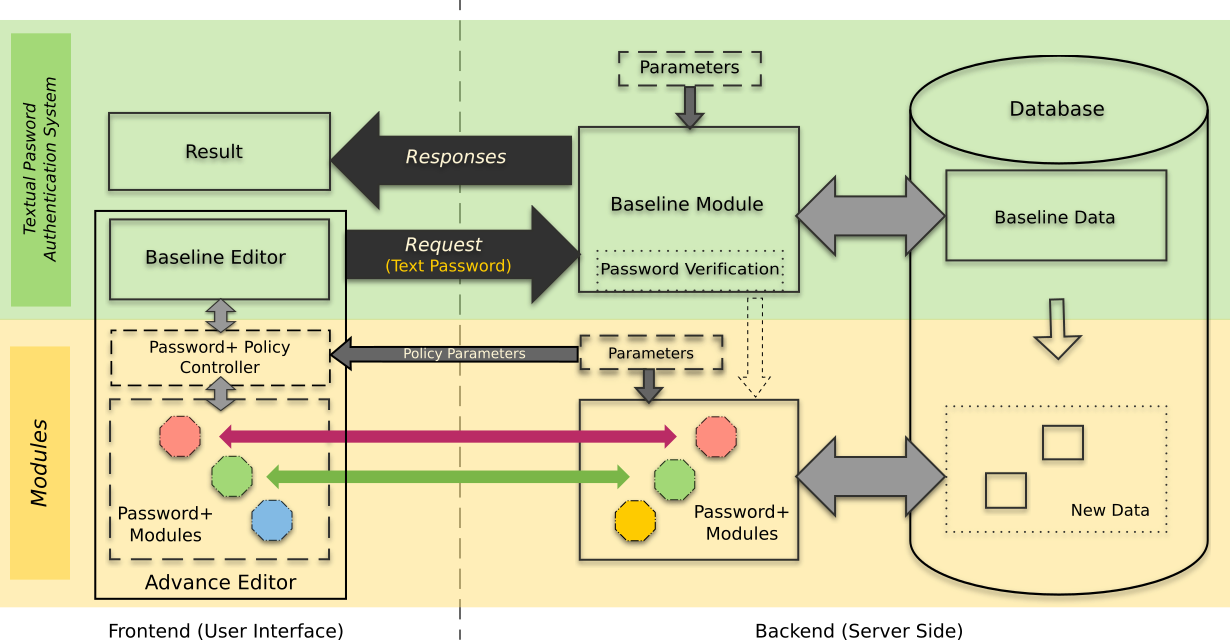
\includegraphics[width=20cm]{figure/architecture.png}
\caption{PassInfinity architecture}
\label{appendix:fig:passarchitecture}
\end{center}
\end{figure}
\end{landscape}

\begin{figure}[!ht]
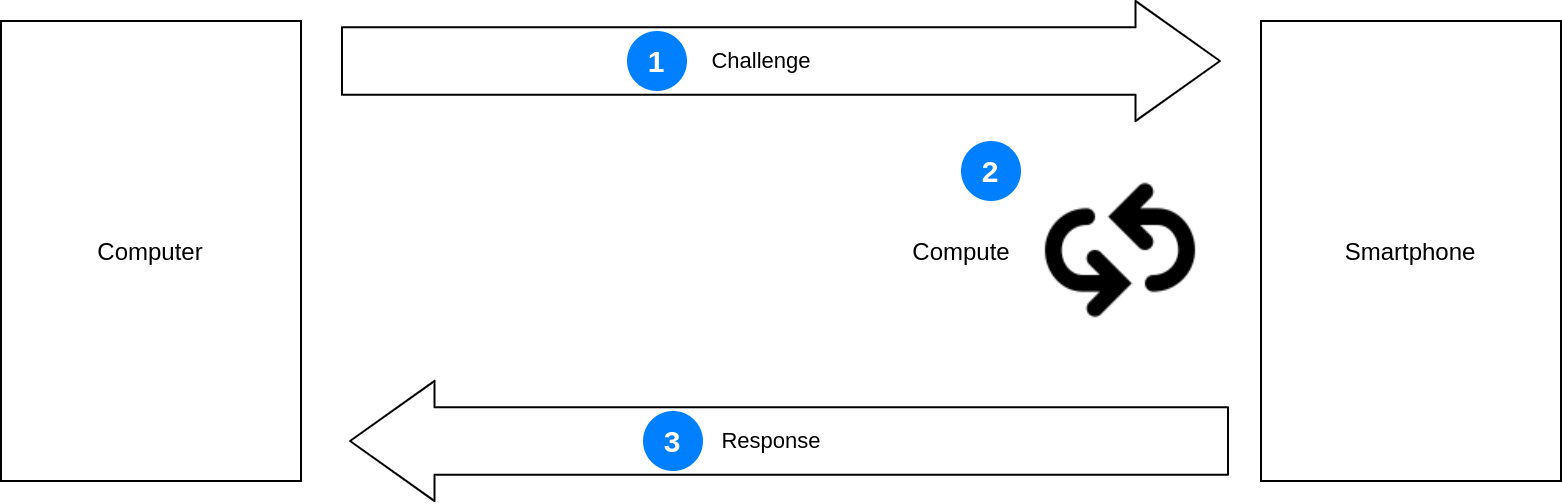
\includegraphics[width=1\textwidth]{figure/audiotokenarchitecture.png}
\caption{Audio Token architecture}
\label{appendix:fig:audioarchitecture}
\end{figure}

\begin{figure}[!ht]
\begin{center}
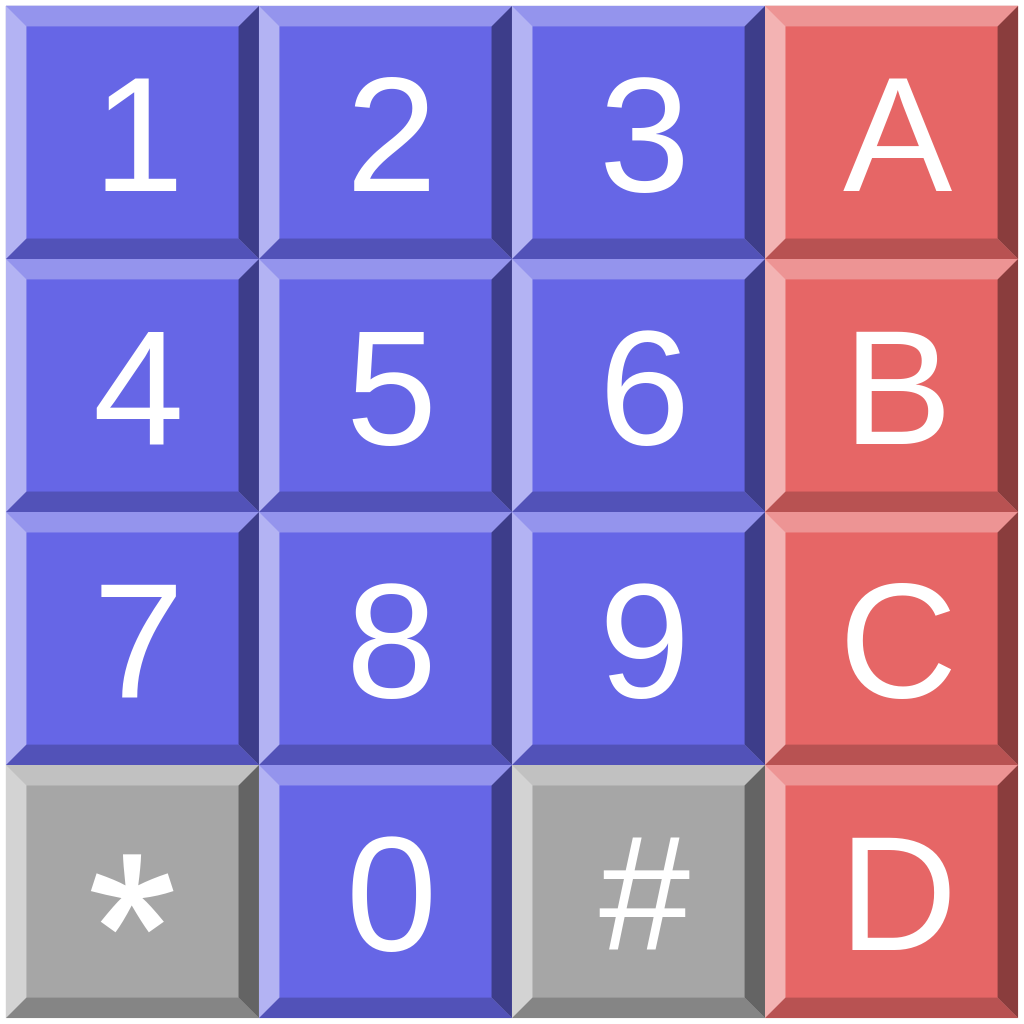
\includegraphics[width=0.6\textwidth]{figure/dtmfkeypad.png}
\caption{A DTMF keypad, source: wikipedia.org}
\label{appendix:fig:dtmfkeypad}
\end{center}
\end{figure}

\begin{figure}[!ht]
\begin{center}
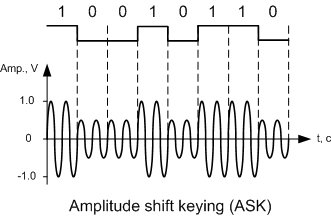
\includegraphics[width=0.6\textwidth]{figure/ask.jpg}
\caption{Amplitude shift keying example, source tmatlantic.com}
\label{appendix:fig:ask}
\end{center}
\end{figure}

\begin{figure}[!ht]
\begin{center}
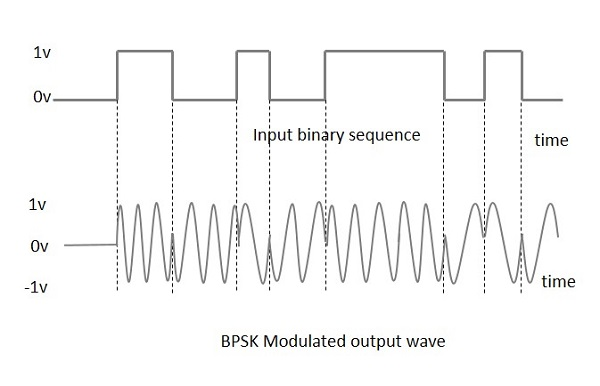
\includegraphics[width=0.6\textwidth]{figure/psk.jpg}
\caption{Phase shift keying example, source: tutorialspoint.com}
\label{appendix:fig:psk}
\end{center}
\end{figure}

\begin{figure}[!ht]
\begin{center}
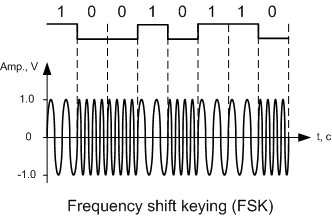
\includegraphics[width=0.6\textwidth]{figure/fsk.jpg}
\caption{Frequency shift keying example, source: tmatlantic.com}
\label{appendix:fig:fsk}
\end{center}
\end{figure}

\begin{figure}[!ht]
\begin{center}
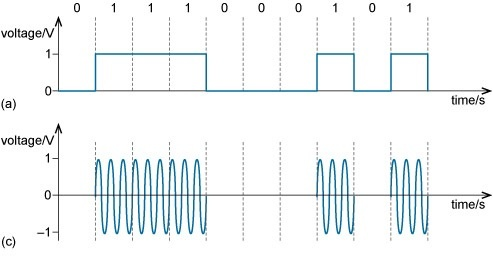
\includegraphics[width=0.6\textwidth]{figure/ook.png}
\caption{On-off keying example, source: open.edu}
\label{appendix:fig:ook}
\end{center}
\end{figure}

\begin{table*}[p]
  \centering
\begin{tabular}{|c|c|c|c|c|}
\hline 
• & 1209 Hz & 1336 Hz & 1477 Hz & 1633 Hz \\ 
\hline 
697 Hz & 1 & 2 & 3 & A \\ 
\hline 
770 Hz & 4 & 5 & 6 & B \\ 
\hline 
852 Hz & 7 & 8 & 9 & C \\ 
\hline 
941 Hz & * & 0 & \# & D \\ 
\hline 
\end{tabular}
\caption{DTMF encode/decode matrix}
\label{appendix:table:dtmf}
\end{table*}

\begin{figure}[!ht]
\begin{lstlisting}[language=JavaScript]
const audioCtx = new window.AudioContext();
\end{lstlisting}
\caption{A code example to instantiate the audio context}
\label{appendix:fig:audioctxinstance}
\end{figure}

\begin{figure}[!ht]
\begin{center}
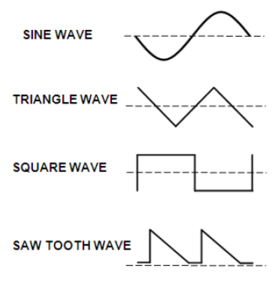
\includegraphics[width=0.5\textwidth]{figure/freqwaveform.png}
\caption{Different frequency waveform shape, source: nerdaudio.com}
\label{appendix:fig:waveformshape}
\end{center}
\end{figure}

\begin{figure}[!ht]
\begin{center}
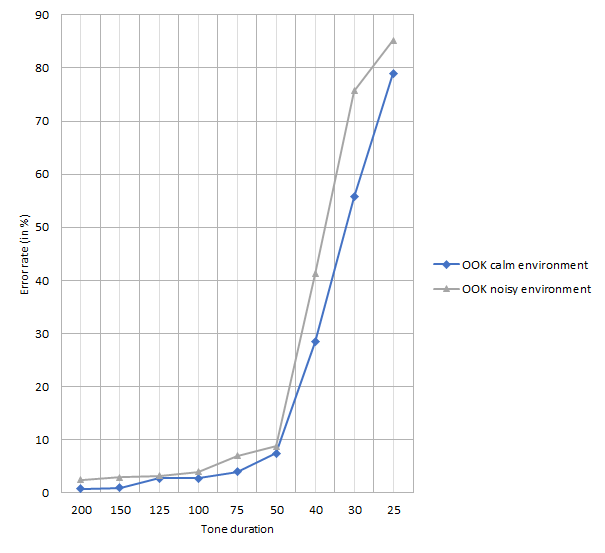
\includegraphics[width=1\textwidth]{figure/ook-graph.png}
\caption{The evolution of the error rate according to the tone duration used for the OOK data transmission algorithm}
\label{appendix:fig:ookgraph}
\end{center}
\end{figure}

\begin{figure}[!ht]
\begin{center}
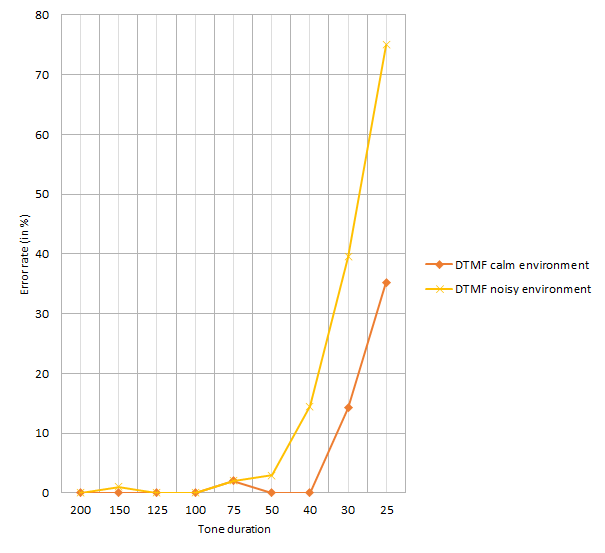
\includegraphics[width=1\textwidth]{figure/dtmf-graph.png}
\caption{The evolution of the error rate according to the tone duration used for the DTMF data transmission algorithm}
\label{appendix:fig:dtmfgraph}
\end{center}
\end{figure}

\begin{figure}[!ht]
\begin{lstlisting}[language=JavaScript]
navigator.getUserMedia({
    audio: true,
}, function(stream) {
    // handle success here
}, function() {
    // handle error here
});
\end{lstlisting}
\caption{A code example to request microphone access}
\label{appendix:fig:requestmicro}
\end{figure}

\begin{figure}[!ht]
\begin{lstlisting}[language=JavaScript]
// Will compute the SHA-256 of the message "hello" (in ASCII)
const toHash = new Uint8Array([104, 101, 108, 108, 111]);
const hash = await window.crypto.subtle.digest('SHA-256', toHash);


// Create a key for HMAC SHA-256
const key = await window.crypto.subtle.generateKey(
	{
		name: 'HMAC',
		hash: {name: 'SHA-256'},
	},
	true,      // indicates whether this key be exported or not
	['sign']   // indicates that this key can only be used with the sign function
	
	
// Use the previously created key to HMAC the message "hello" (in ASCII)
const hmac = await window.crypto.subtle.sign('HMAC', key, toHash);
\end{lstlisting}
\caption{Some code examples of the Web Crypto API}
\label{appendix:fig:cryptoapiex}
\end{figure}

\end{document}